\chapter{Experiments}
\section{Dropout Experiment}


\begin{figure}[ht]
   \centering
   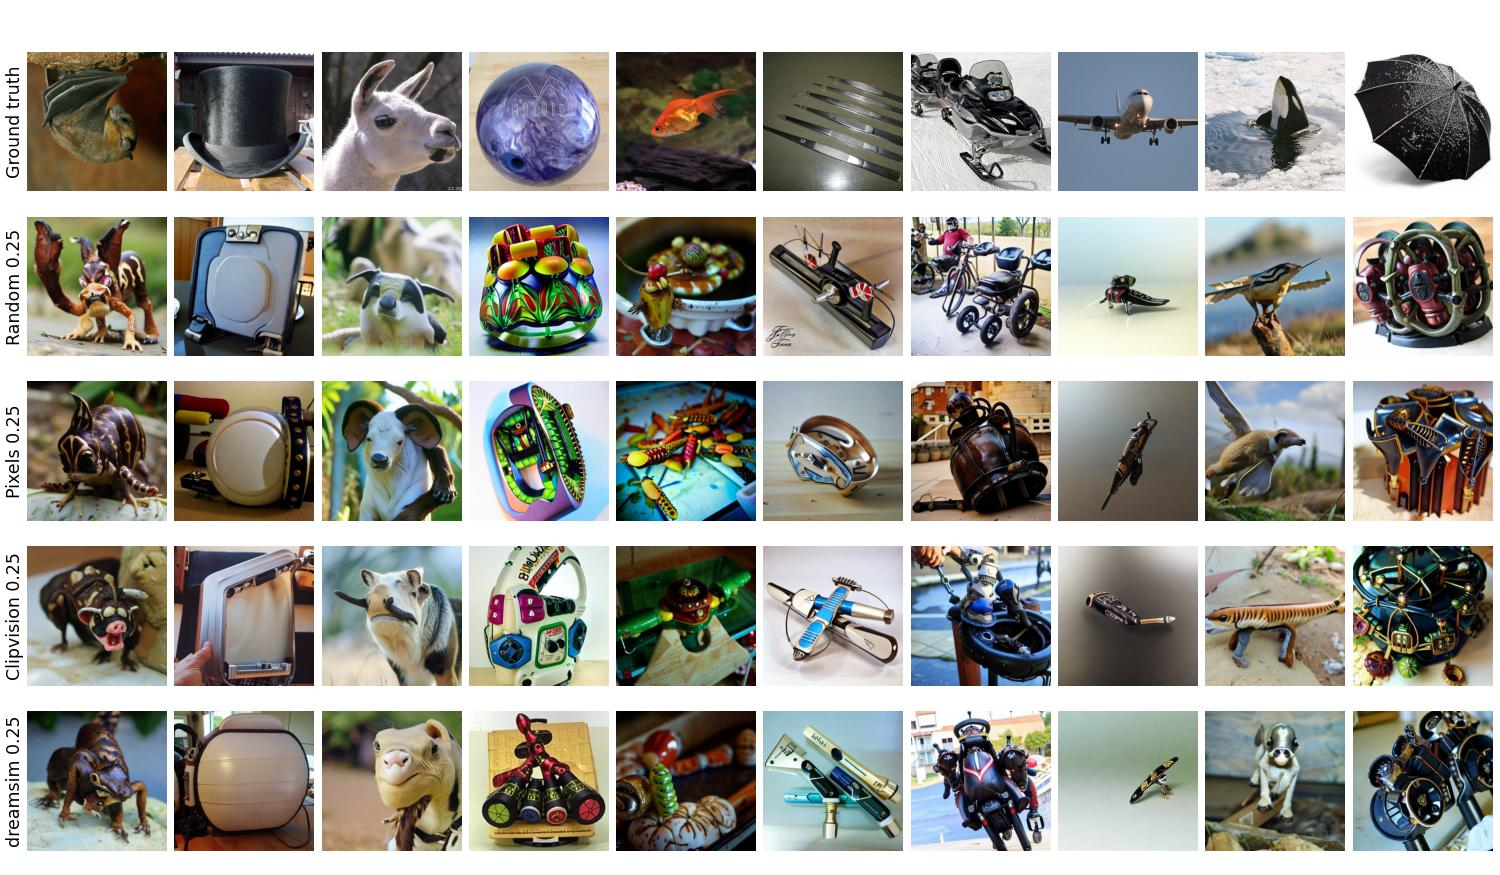
\includegraphics[width=1\textwidth]{plots/dropout_qual_eval_bd_test.JPEG}
   \caption{A nice image}\label{fig:dropout_qual_eval_bd_test}
\end{figure}

\begin{figure}[ht]
   \centering
   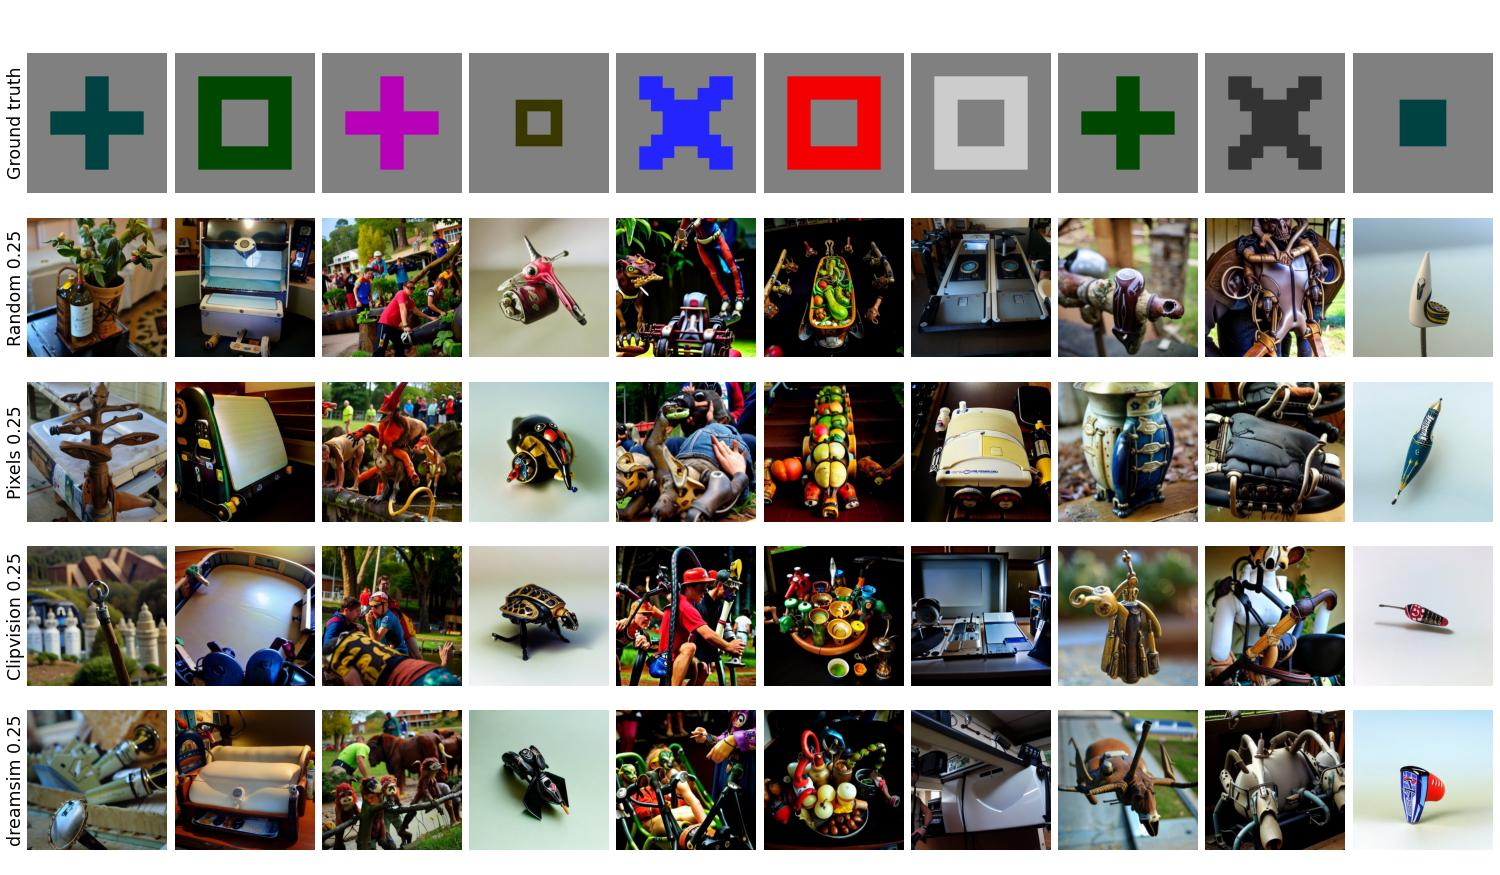
\includegraphics[width=1\textwidth]{plots/dropout_qual_eval_bd_art.JPEG}
   \caption{A nice image}\label{fig:dropout_qual_eval_bd_art}
\end{figure}

\section{Ai Captions}
\begin{figure}[ht]
   \centering
   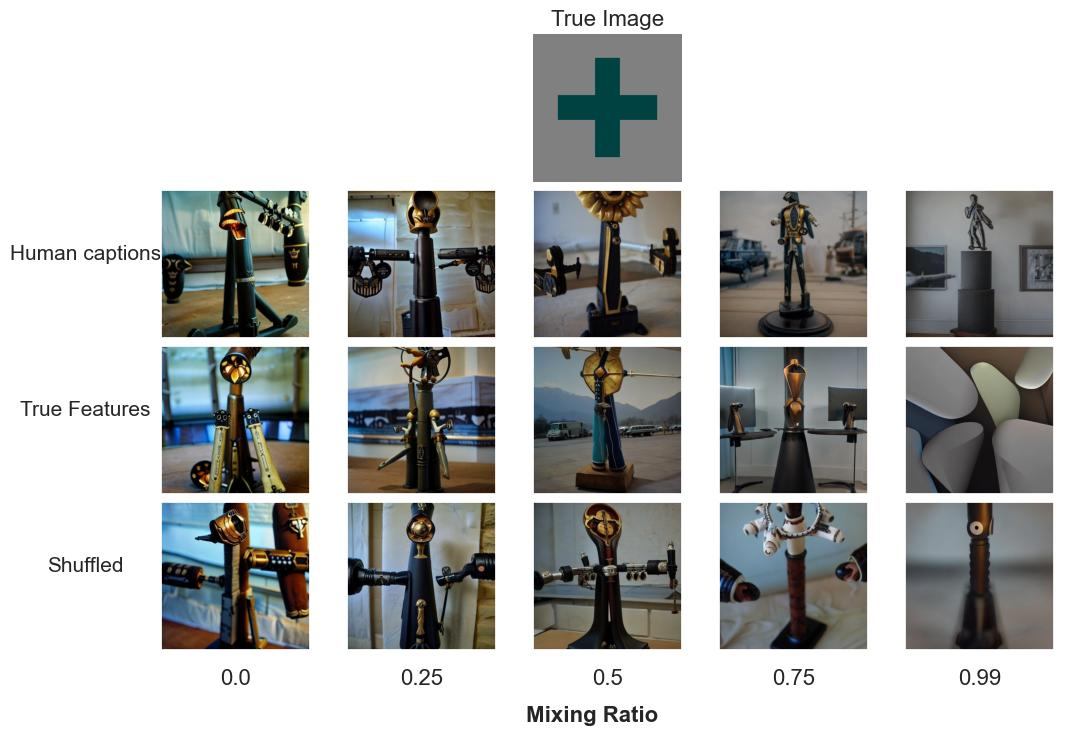
\includegraphics[width=1\textwidth]{plots/aicap_reconstruction_evolution_art_0.JPEG}
   \caption{AI-cap Reconstructions Artificial Shapes}\label{fig:aicap_reconstruction_evolution_art_0}
\end{figure}

\begin{figure}[ht]
   \centering
   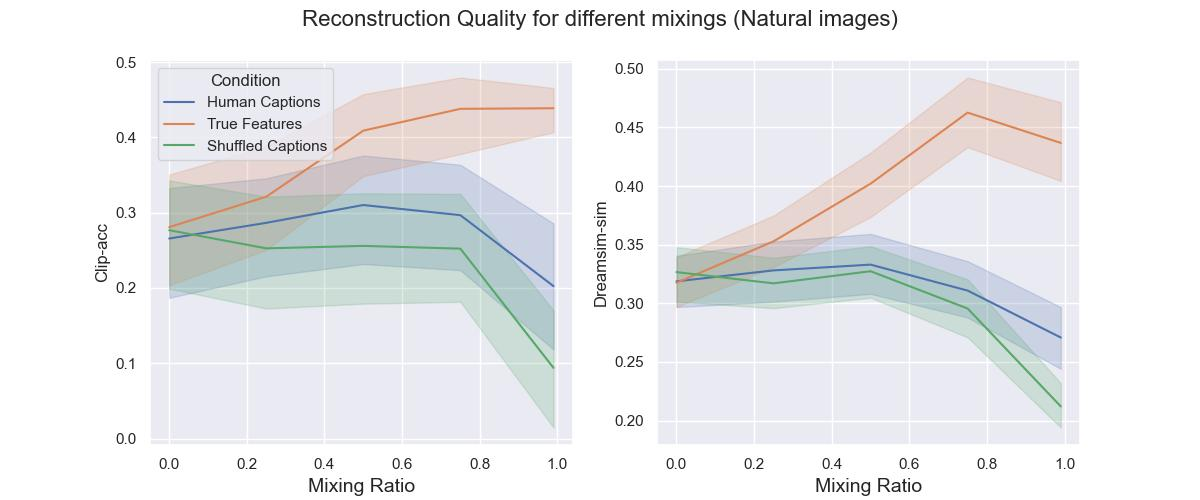
\includegraphics[width=1\textwidth]{plots/aicap_reconstruction_quant_evolution_test.JPEG}
   \caption{AI-cap Reconstructions Artificial Shapes}\label{fig:aicap_reconstruction_quant_evolution_test}
\end{figure}

\begin{figure}[ht]
   \centering
   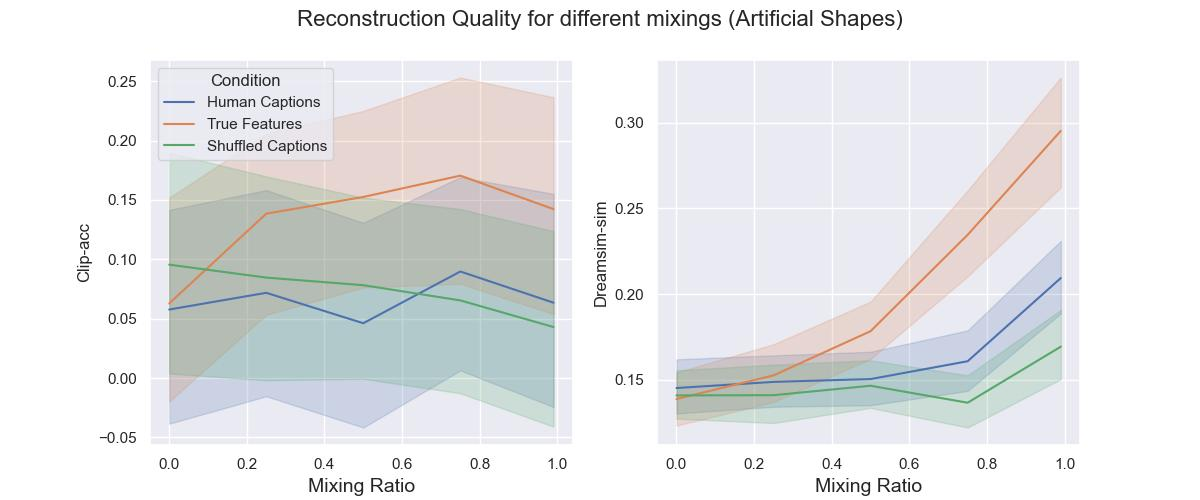
\includegraphics[width=1\textwidth]{plots/aicap_reconstruction_quant_evolution_art.JPEG}
   \caption{AI-cap Reconstructions Artificial Shapes}\label{fig:aicap_reconstruction_quant_evolution_art}
\end{figure}

\section{Perturbations}
\begin{figure}[ht]
    \centering
    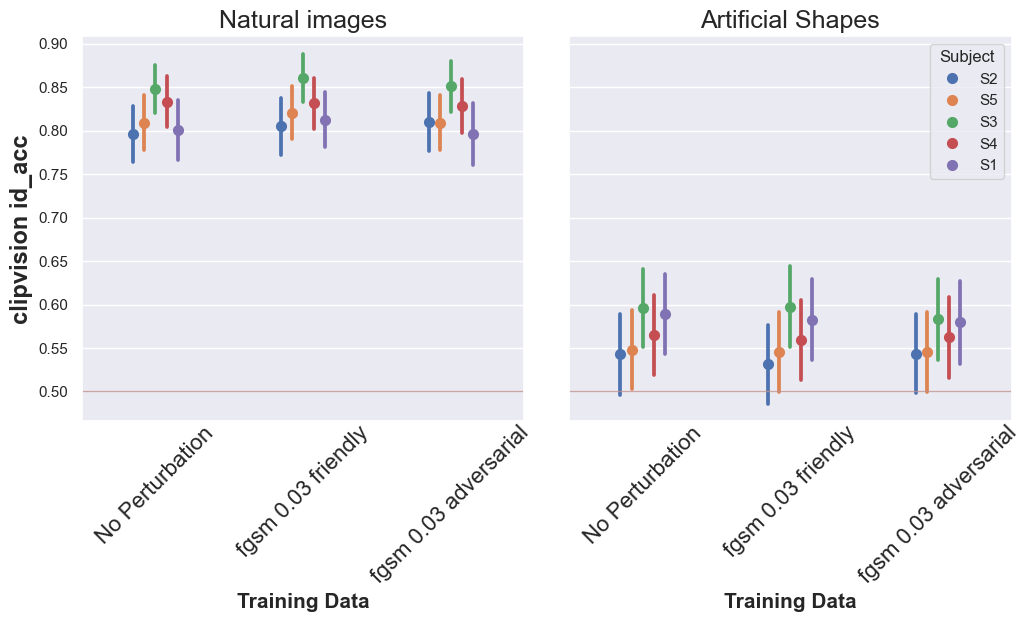
\includegraphics[width=1\textwidth]{plots/advpert_translator_fgsm_0.03.png}
    \caption{FGSM 0.03 Translator Performance}\label{fig:advpert_translator_fgsm_0}
\end{figure}

\begin{figure}[ht]
    \centering
    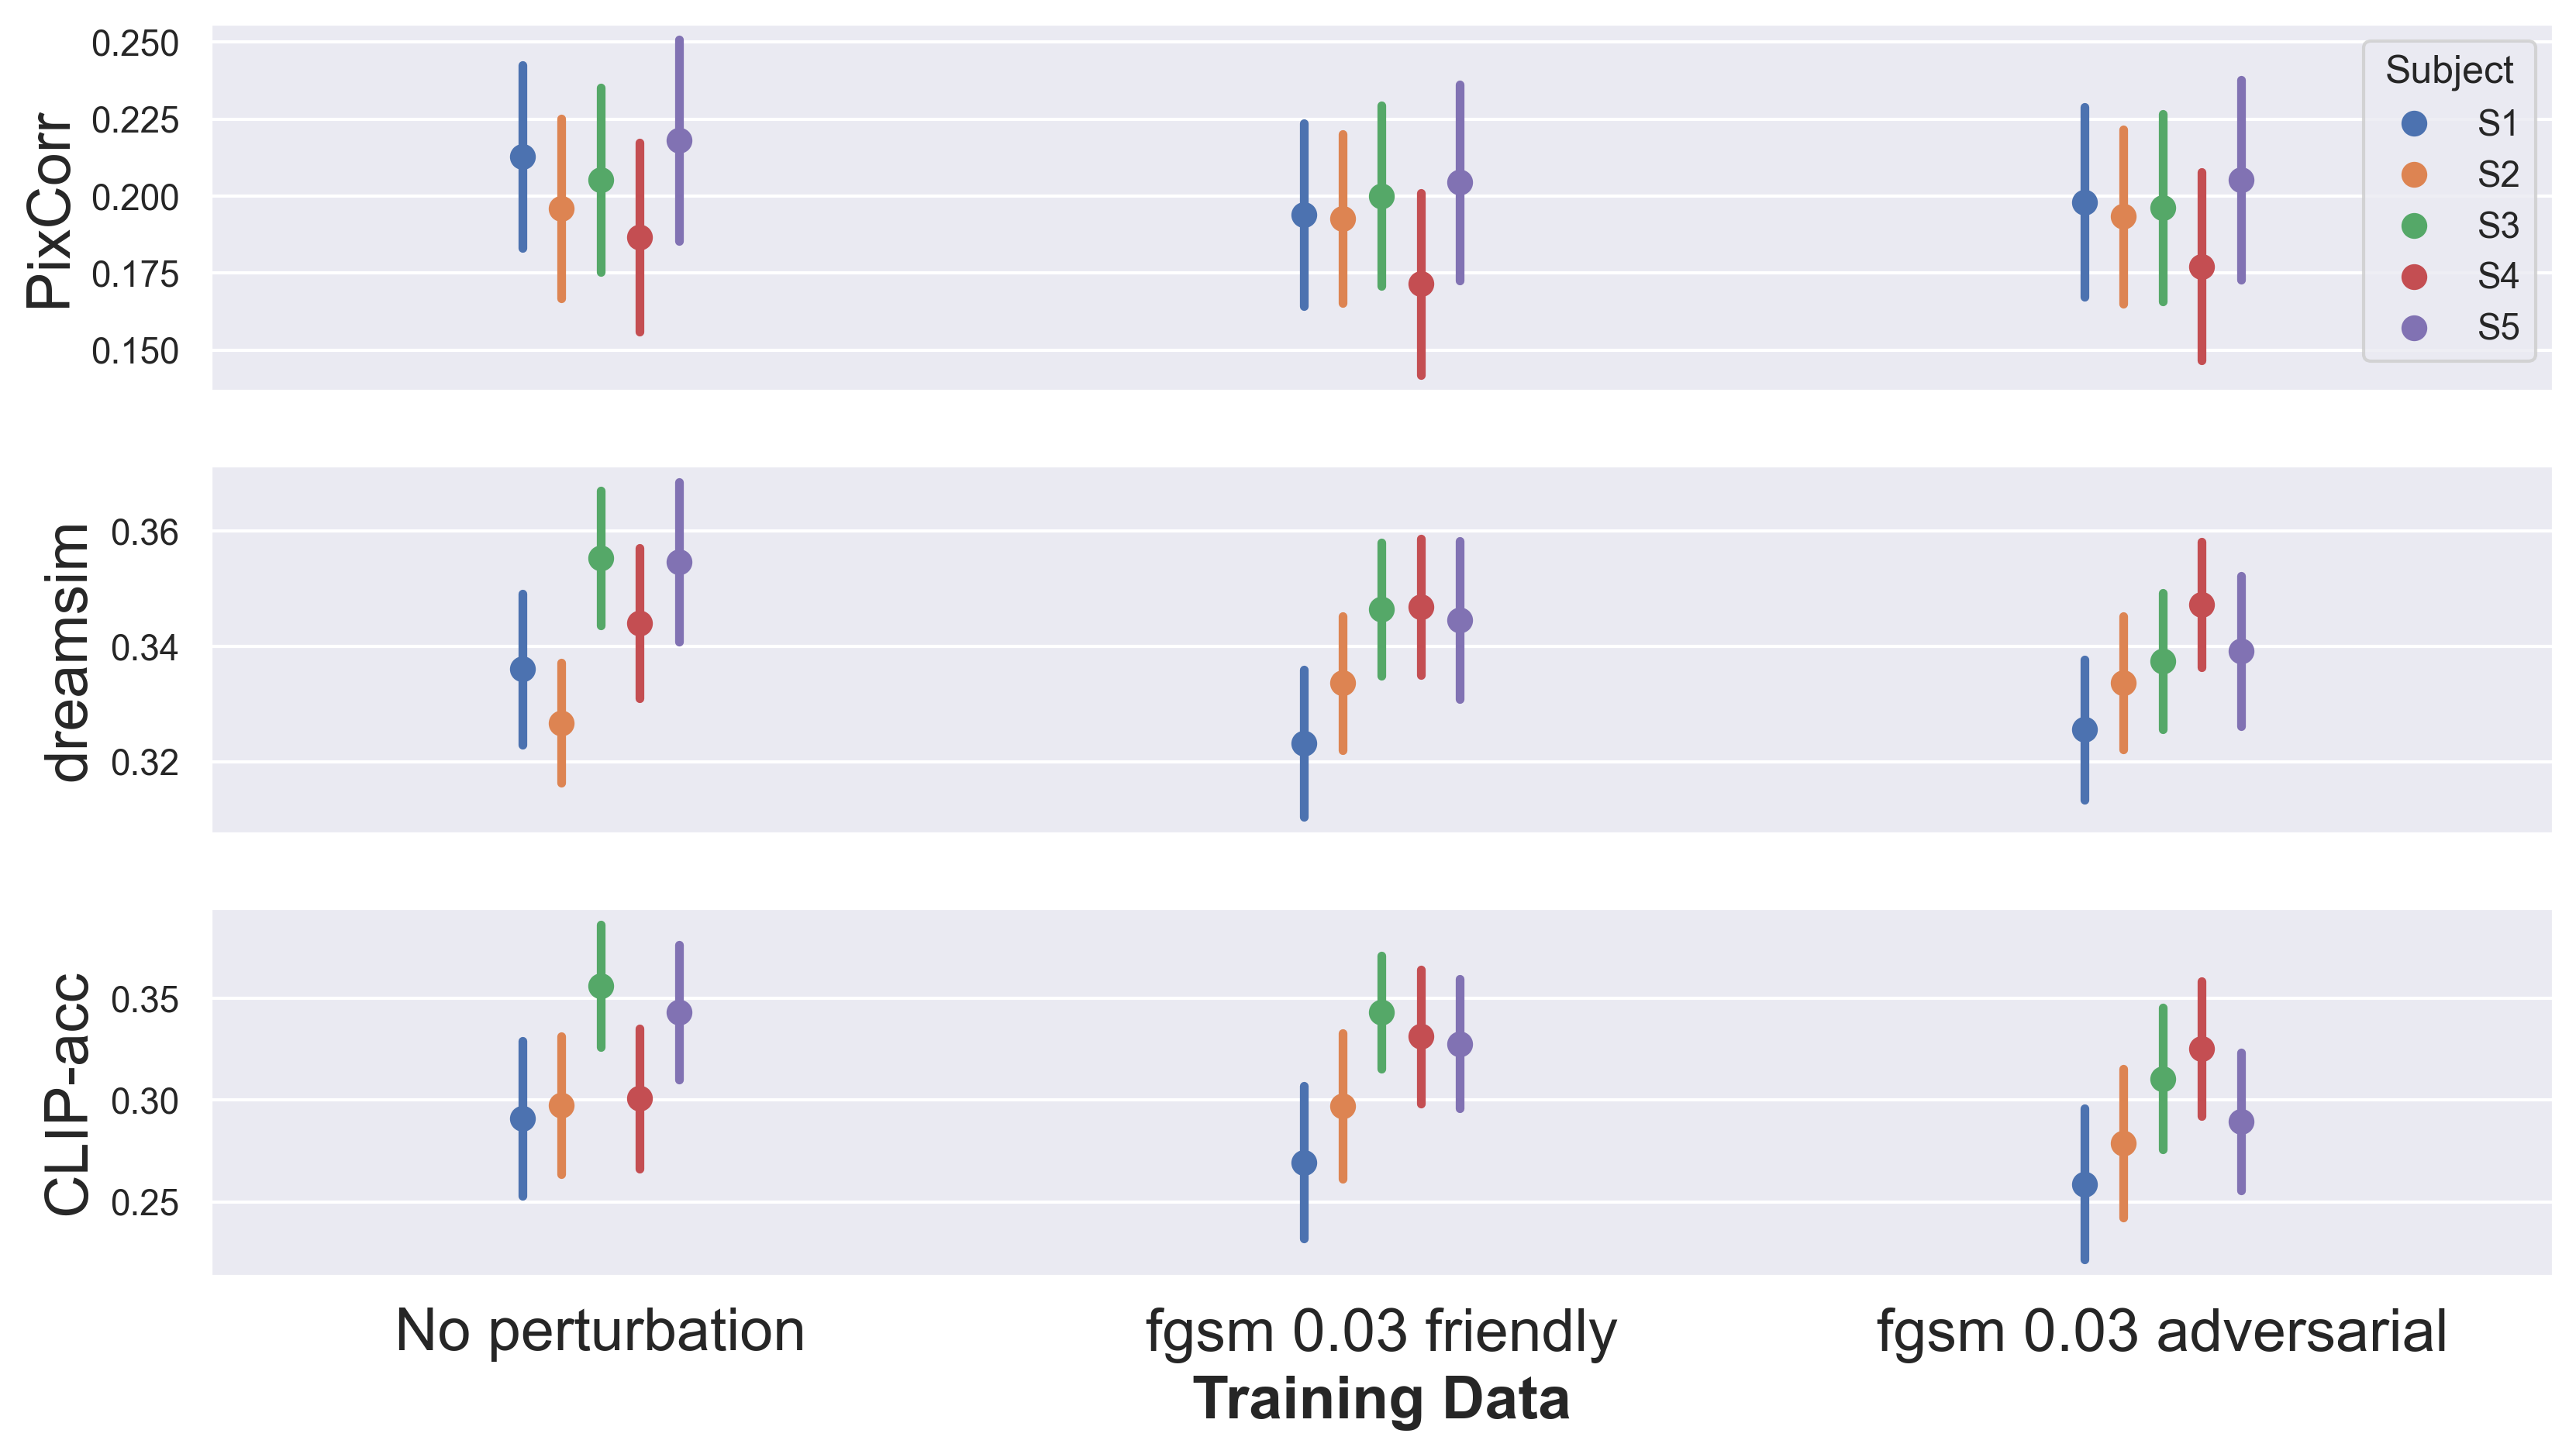
\includegraphics[width=1\textwidth]{plots/advpert_reconstruction_test_fgsm_0.03.png}
    \caption{FGSM 0.03 Reconstruction Performance Natural Test Images}\label{fig:advpert_reconstruction_test_fgsm_0.03}
\end{figure}

\begin{figure}[ht]
    \centering
    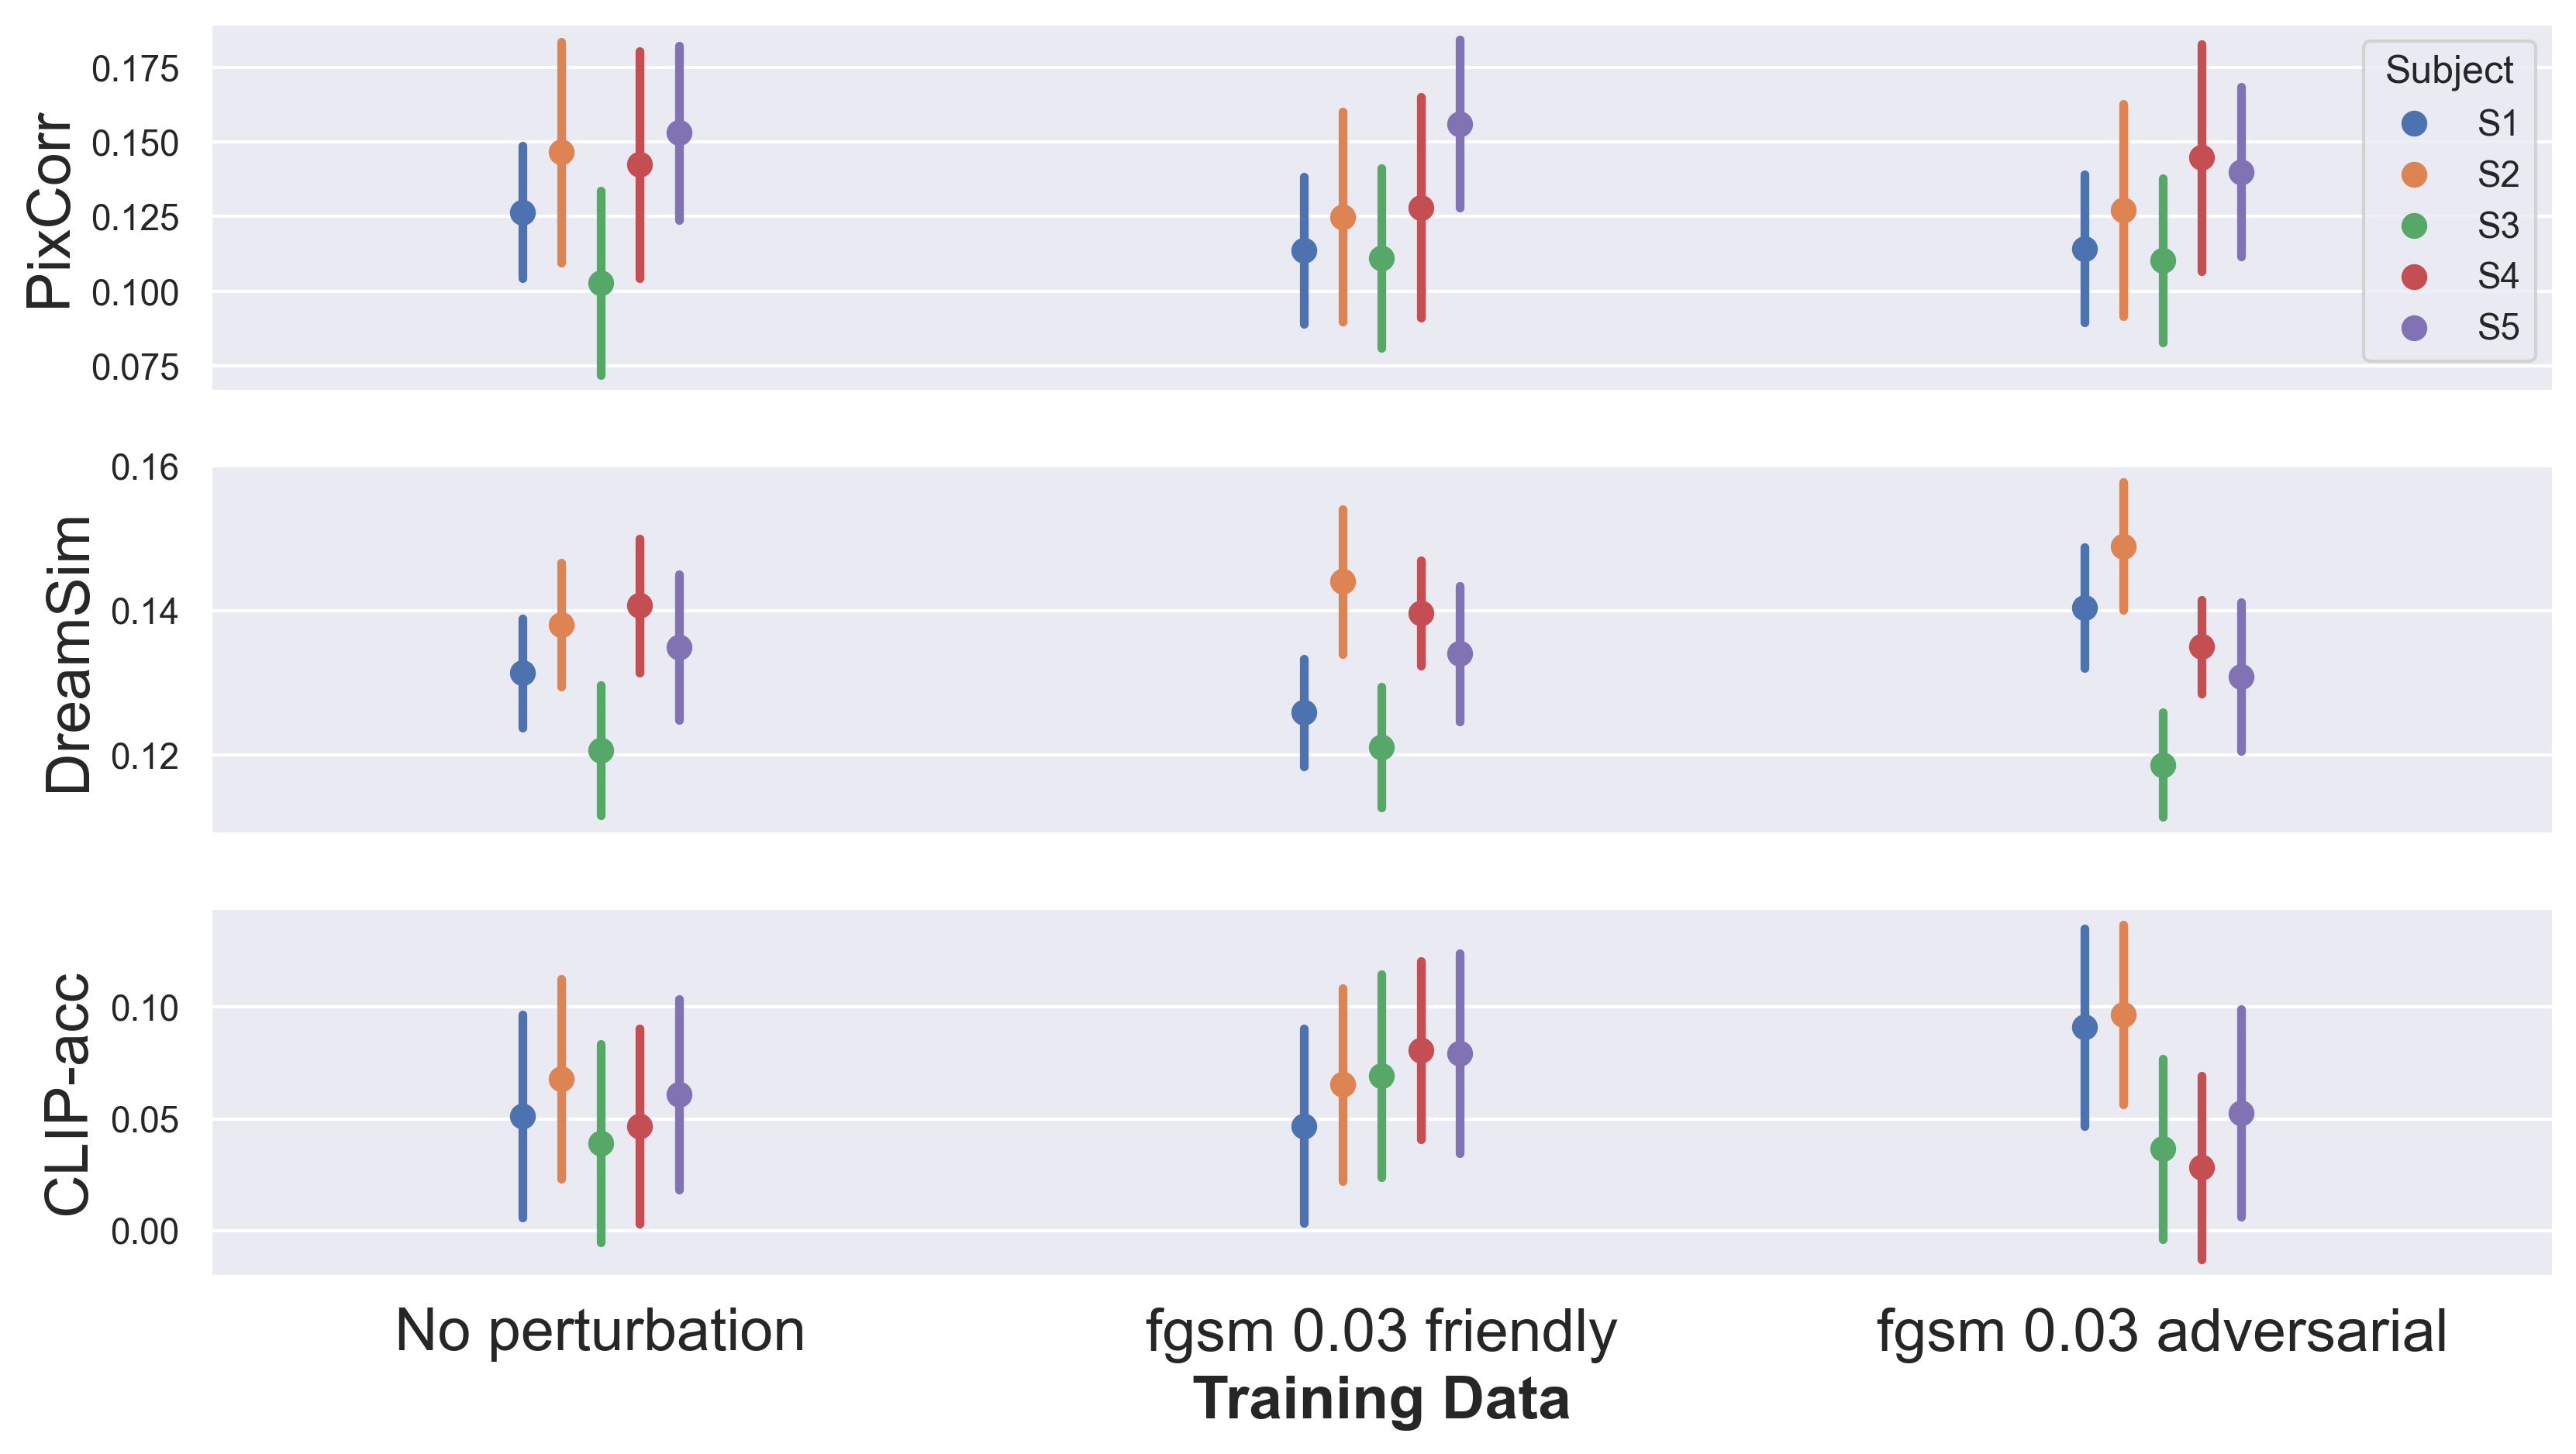
\includegraphics[width=1\textwidth]{plots/advpert_reconstruction_art_fgsm_0.03.png}
    \caption{FGSM 0.03 Reconstruction Performance Artificial Shapes}\label{fig:advpert_reconstruction_art_fgsm_0.03}
\end{figure}

\begin{figure}[ht]
   \centering
   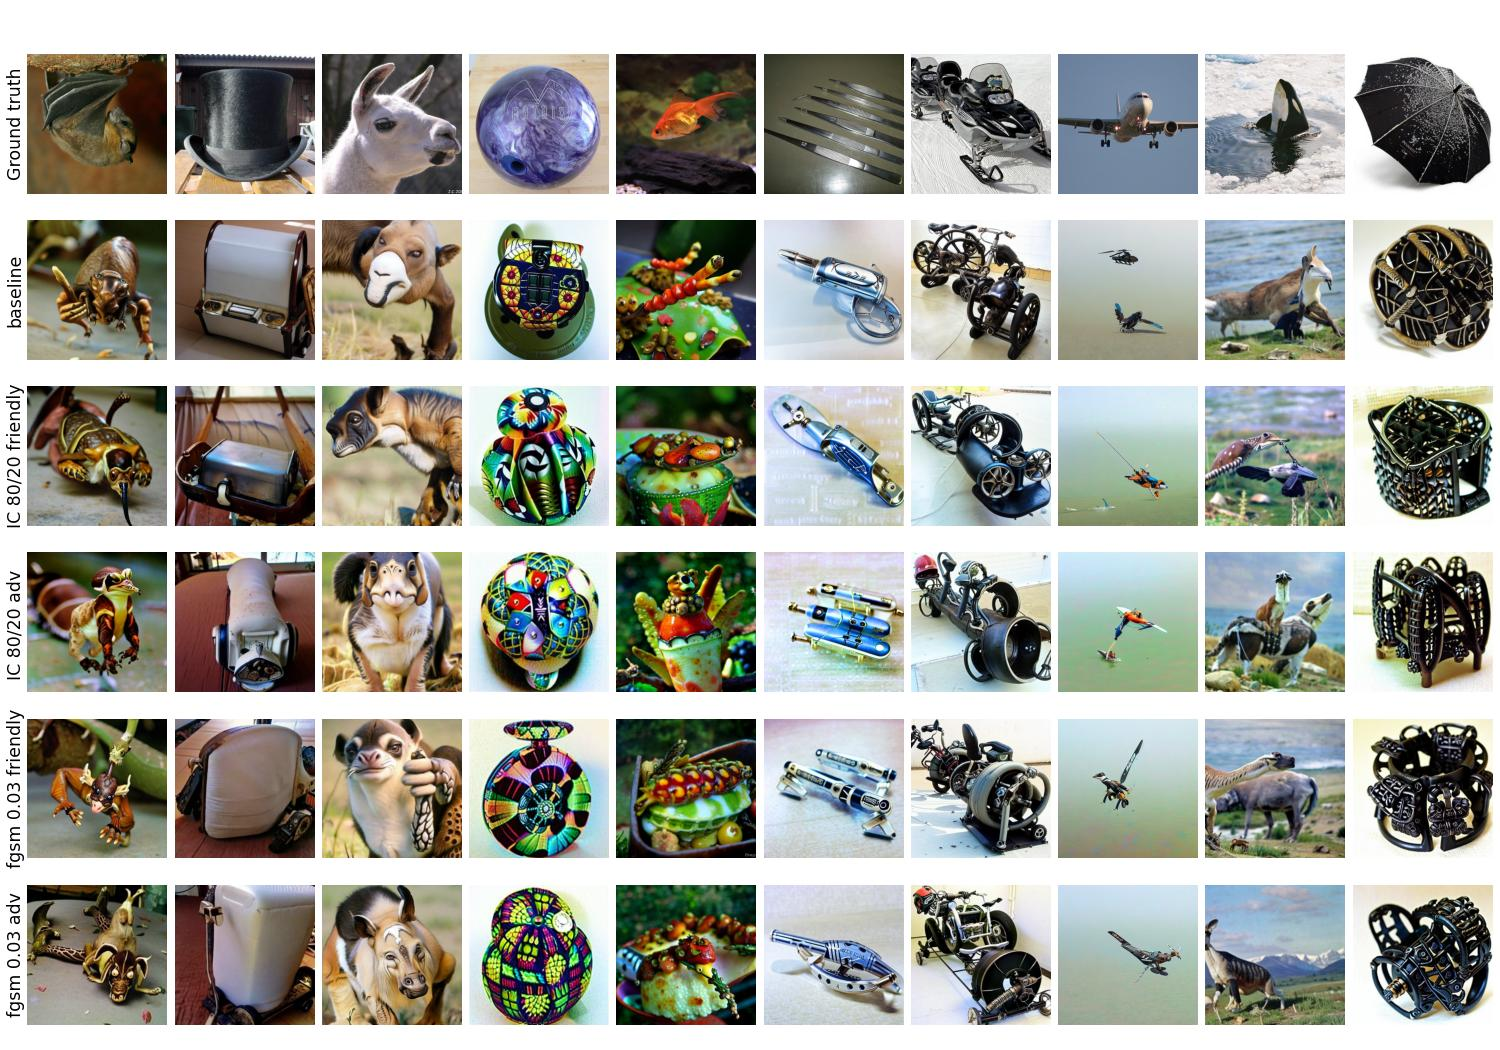
\includegraphics[width=1\textwidth]{plots/advpert_qual_test.JPEG}
   \caption{Qualitative Results for the perturbations experiment Natural Test Images}\label{fig:advpert_qual_test}
\end{figure}

\begin{figure}[ht]
   \centering
   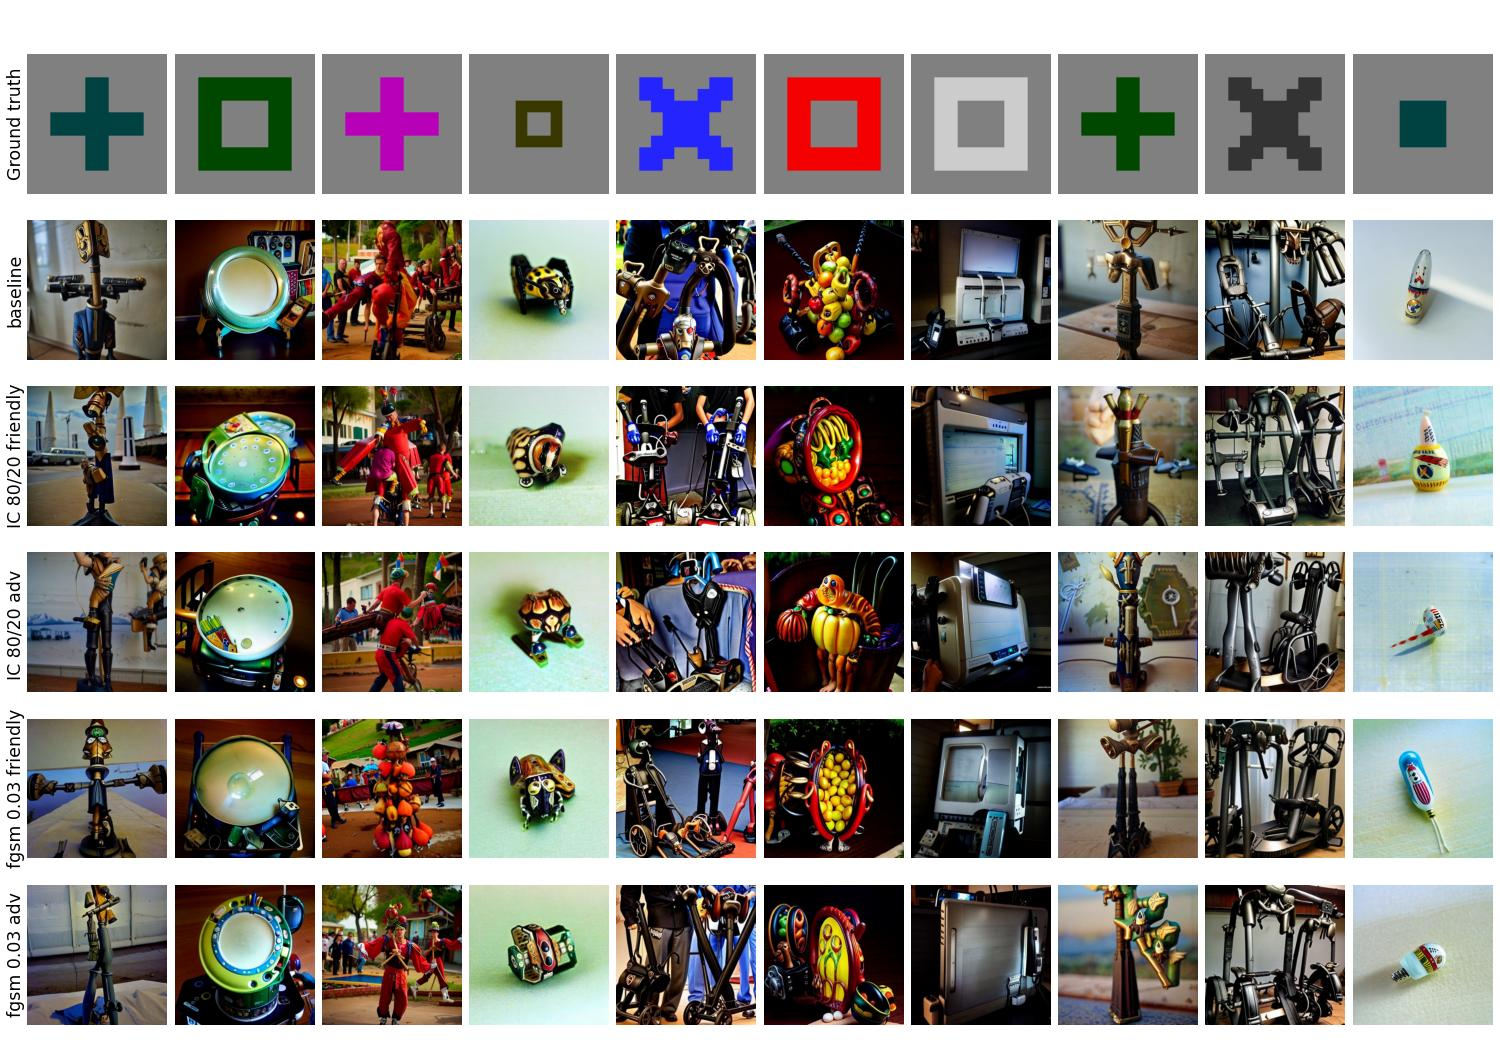
\includegraphics[width=1\textwidth]{plots/advpert_qual_art.JPEG}
   \caption{Qualitative Results for the perturbations experiment Artificial Shapes}\label{fig:advpert_qual_art}
\end{figure}

